\documentclass[aspectratio=169,10pt]{beamer}

\usepackage[utf8]{inputenc}
\usepackage[T1]{fontenc}
\usepackage[spanish,es-nodecimaldot]{babel}
\usepackage{lmodern}
\usepackage{graphicx}
\usepackage{booktabs}
\usepackage{tabularx}
\usepackage{array}
\usepackage{colortbl}
\usepackage{amssymb}
\usepackage{tikz}

\definecolor{FraudBlue}{HTML}{2E6F9E}
\definecolor{FraudDark}{HTML}{263238}
\definecolor{FraudGray}{HTML}{64748B}
\definecolor{FraudLightGray}{HTML}{F1F5F9}
\definecolor{FraudLine}{HTML}{D8E1EA}
\definecolor{FraudPaleBlue}{HTML}{EAF2F8}

\usetheme{default}
\setbeamertemplate{navigation symbols}{}
\setbeamertemplate{headline}{}
\setbeamertemplate{itemize item}{\color{FraudBlue}\scriptsize$\blacktriangleright$}
\setbeamertemplate{itemize subitem}{\color{FraudGray}\tiny$\bullet$}
\setbeamercolor{normal text}{fg=FraudDark,bg=white}
\setbeamercolor{structure}{fg=FraudBlue}
\setbeamercolor{frametitle}{fg=FraudDark,bg=white}
\setbeamerfont{frametitle}{series=\bfseries,size=\large}
\setbeamercolor{block title}{fg=FraudBlue,bg=FraudPaleBlue}
\setbeamercolor{block body}{fg=FraudDark,bg=FraudLightGray}
\setbeamercolor{footline}{fg=FraudGray,bg=white}
\setbeamertemplate{blocks}[rounded][shadow=false]
\setbeamertemplate{frametitle}{%
  \vspace{0.35em}%
  \insertframetitle\par
  \vspace{0.15em}%
  {\color{FraudBlue}\rule{\textwidth}{0.55pt}}%
}
\setbeamertemplate{footline}{%
  \begin{beamercolorbox}[wd=\paperwidth,ht=2.5ex,dp=1.1ex,leftskip=0.65cm,rightskip=0.65cm]{footline}%
    \scriptsize INFO1185 -- Detección de fraude
    \hfill \insertframenumber/\inserttotalframenumber
  \end{beamercolorbox}%
}
\setlength{\tabcolsep}{5pt}
\renewcommand{\arraystretch}{1.18}
\graphicspath{{../../resultados/graficos/}}

\newcommand{\metricbox}[2]{%
  \begin{beamercolorbox}[wd=\linewidth,sep=0.55em,center,rounded=true]{block body}%
    {\color{FraudBlue}\Large\bfseries #1}\par\vspace{0.12em}
    {\small #2}
  \end{beamercolorbox}%
}
\newcommand{\cvrow}[5]{#1 & #2 & #3 & #4 & #5\\}

\title[Detección de fraude]{Detección de fraude con aprendizaje supervisado}
\subtitle{Comparación de clasificadores y prioridad en reducir falsos negativos}
\author{Fernando Valdés Gomez \and Juan Muñoz Veloso}
\institute{INFO1185 \textbullet\ Inteligencia Artificial}
\date{9 de octubre de 2026}

\begin{document}

% 1. Portada
\begin{frame}[plain]
  \vspace{0.85cm}
  {\color{FraudBlue}\small\bfseries INFO1185 -- INTELIGENCIA ARTIFICIAL}\par
  \vspace{0.8cm}
  {\Huge\bfseries\color{FraudDark} Detección de fraude}\par
  \vspace{0.25cm}
  {\Large\color{FraudGray} Comparación de clasificadores supervisados}\par
  \vspace{0.8cm}
  {\color{FraudBlue}\rule{0.62\textwidth}{1.2pt}}\par
  \vspace{0.35cm}
  {\large Prioridad: detectar fraudes y reducir falsos negativos}\par
  \vfill
  \begin{columns}[T,onlytextwidth]
    \column{0.56\textwidth}
      \normalsize Fernando Valdés Gomez\\ Juan Muñoz Veloso
    \column{0.4\textwidth}
      \raggedleft\color{FraudGray} 4 clasificadores -- 8 condiciones
  \end{columns}
  \vspace{0.55cm}
\end{frame}

% 2. Datos
\begin{frame}{El fraude es poco frecuente}
  \begin{columns}[T,onlytextwidth]
    \column{0.63\textwidth}
      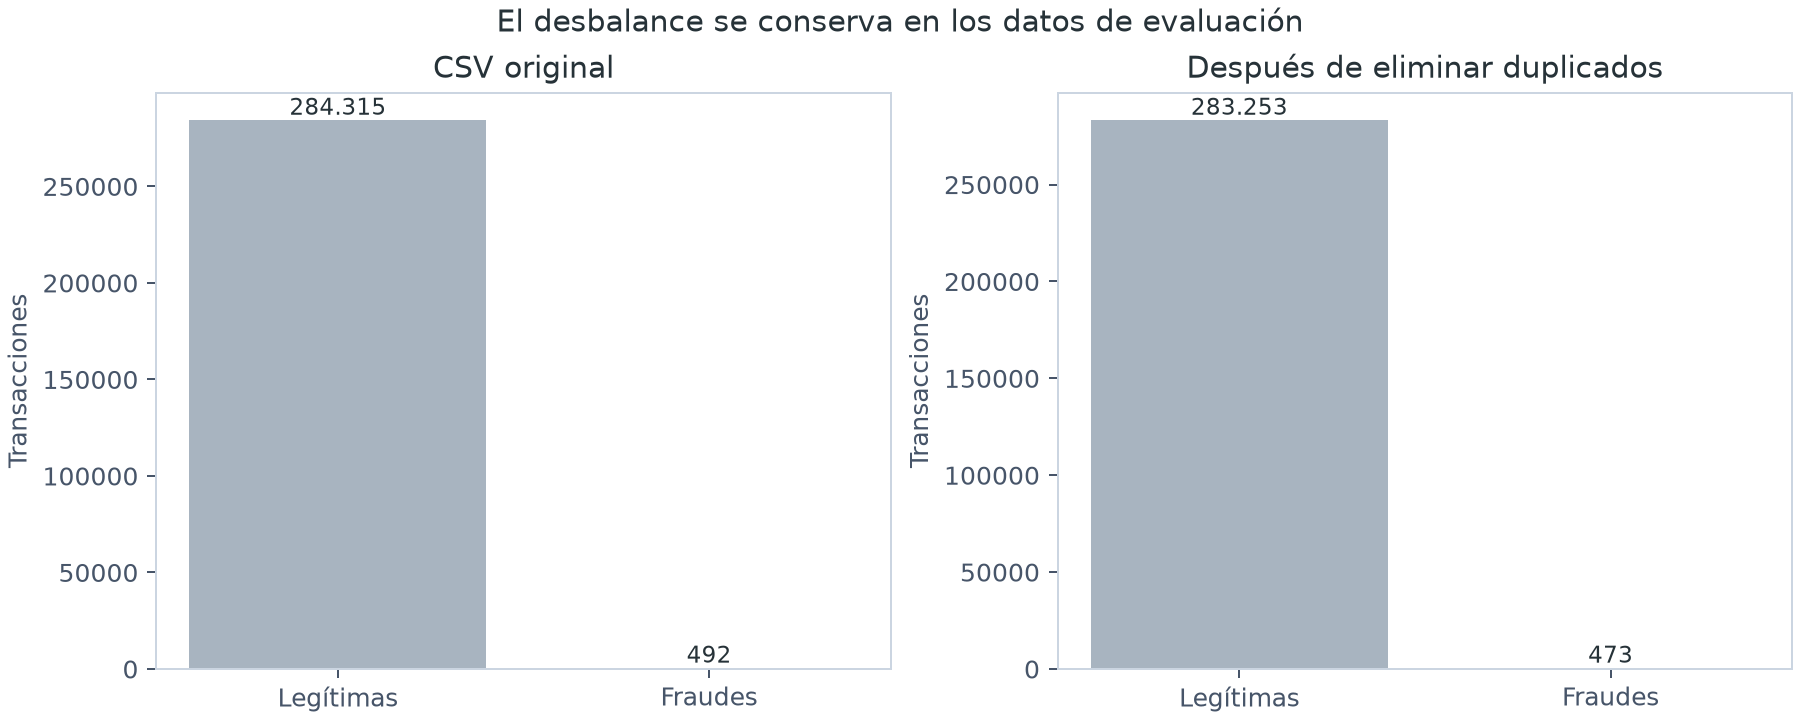
\includegraphics[width=\linewidth,height=0.64\textheight,keepaspectratio]{distribucion_clases.png}
    \column{0.34\textwidth}
      \begin{block}{Datos originales}
        \begin{itemize}
          \item 284.807 transacciones.
          \item 492 fraudes (0,173\%).
          \item 30 variables predictoras.
        \end{itemize}
      \end{block}
      \vspace{0.15cm}
      \begin{block}{Limpieza}
        1.081 duplicados exactos eliminados; cero valores faltantes.\\[0.15em]
        Quedaron 283.726 filas y 473 fraudes.
      \end{block}
  \end{columns}
\end{frame}

% 3. Partición y fuga
\begin{frame}{Partición fija y prueba reservada}
  \begin{columns}[T,onlytextwidth]
    \column{0.32\textwidth}\metricbox{198.608}{filas de entrenamiento completo}
    \column{0.32\textwidth}\metricbox{50.000}{filas estratificadas para búsqueda}
    \column{0.32\textwidth}\metricbox{85.118}{filas en prueba reservada}
  \end{columns}
  \vspace{0.5cm}
  \begin{block}{Protocolo}
    \begin{itemize}
      \item División estratificada 70/30 con semilla 42; los ocho experimentos comparten la misma partición.
      \item Búsqueda con cinco pliegues estratificados compartidos sobre una submuestra fija del entrenamiento.
      \item Cada ganador se reajusta con todo el entrenamiento antes de evaluar la prueba.
      \item La prueba conserva la prevalencia natural y no participa en ningún ajuste.
    \end{itemize}
  \end{block}
\end{frame}

% 4. Matriz experimental y pipeline
\begin{frame}{Ocho experimentos, una misma validación}
  \begin{columns}[T,onlytextwidth]
    \column{0.44\textwidth}
      \begin{block}{Matriz de comparación}
        \small
        \textbf{Modelos}\par\vspace{0.1cm}
        k-NN, árbol de decisión, SVM lineal y Random Forest propio.
        \vspace{0.25cm}

        \textbf{Condiciones por modelo}\par\vspace{0.1cm}
        Sin compensación y con submuestreo aleatorio 1:10.\\[0.25em]
        \textcolor{FraudBlue}{\bfseries 4 modelos $\times$ 2 condiciones = 8 experimentos}
      \end{block}
    \column{0.52\textwidth}
      \begin{block}{Dentro de cada pliegue}
        \begin{itemize}
          \item Escalado estándar para k-NN y SVM.
          \item ANOVA F-test: selección de 20 de 30 variables.
          \item RandomUnderSampler con proporción 1:10 solo en entrenamiento.
          \item Validación y prueba no se remuestrean.
        \end{itemize}
      \end{block}
  \end{columns}
\end{frame}

% 5. Random Forest
\begin{frame}{Random Forest implementado para el proyecto}
  \begin{columns}[T,onlytextwidth]
    \column{0.32\textwidth}
      \begin{block}{1. Bootstrap}
        Para cada árbol, extraer $n$ filas con reemplazo desde el entrenamiento disponible.
      \end{block}
    \column{0.32\textwidth}
      \begin{block}{2. Árbol independiente}
        Usar \texttt{DecisionTreeClassifier}; elegir $\sqrt{p}$ variables candidatas en cada división.
      \end{block}
    \column{0.32\textwidth}
      \begin{block}{3. Votación}
        Combinar predicciones por mayoría. En empate, asignar clase fraude.
      \end{block}
  \end{columns}
  \vspace{0.45cm}
  \begin{center}
    \large Configuración elegida: \texttt{n\_estimators=21}, \texttt{max\_depth=6}
  \end{center}
  \begin{center}\small No se utilizan \texttt{RandomForestClassifier} ni \texttt{BaggingClassifier}.\end{center}
\end{frame}

% 6. Selección
\begin{frame}{Selección por sensibilidad y precisión}
  \begin{columns}[T,onlytextwidth]
    \column{0.56\textwidth}
      \begin{block}{Regla de selección}
        \begin{enumerate}
          \item Maximizar la sensibilidad media de la clase fraude en cinco pliegues.
          \item Si hay empate, elegir mayor precisión media de fraude.
        \end{enumerate}
        \vspace{0.2cm}
        Elegida: \textbf{Random Forest propio con submuestreo 1:10}.\\
        Sensibilidad CV: \textbf{87,9\% $\pm$ 5,5\%}; precisión: \textbf{45,0\%}.
      \end{block}
    \column{0.41\textwidth}
      \begin{block}{Búsqueda acotada}
        \small
        k-NN: $k\in\{3,5,7\}$.\\
        Árbol: profundidad $\{5,10,\text{sin límite}\}$; hojas $\{1,5\}$.\\
        SVM lineal: $C\in\{0{,}1;\ 1;\ 10\}$.\\
        Bosque: árboles $\{11,21\}$; profundidad $\{6,12\}$.
      \end{block}
  \end{columns}
  \vspace{0.15cm}
  \centering\scriptsize Selección ANOVA de las 20 variables y parámetros ajustados solo dentro del entrenamiento de cada pliegue.
\end{frame}

% 7. Validación
\begin{frame}{Validación cruzada: detección de fraude}
  \centering
  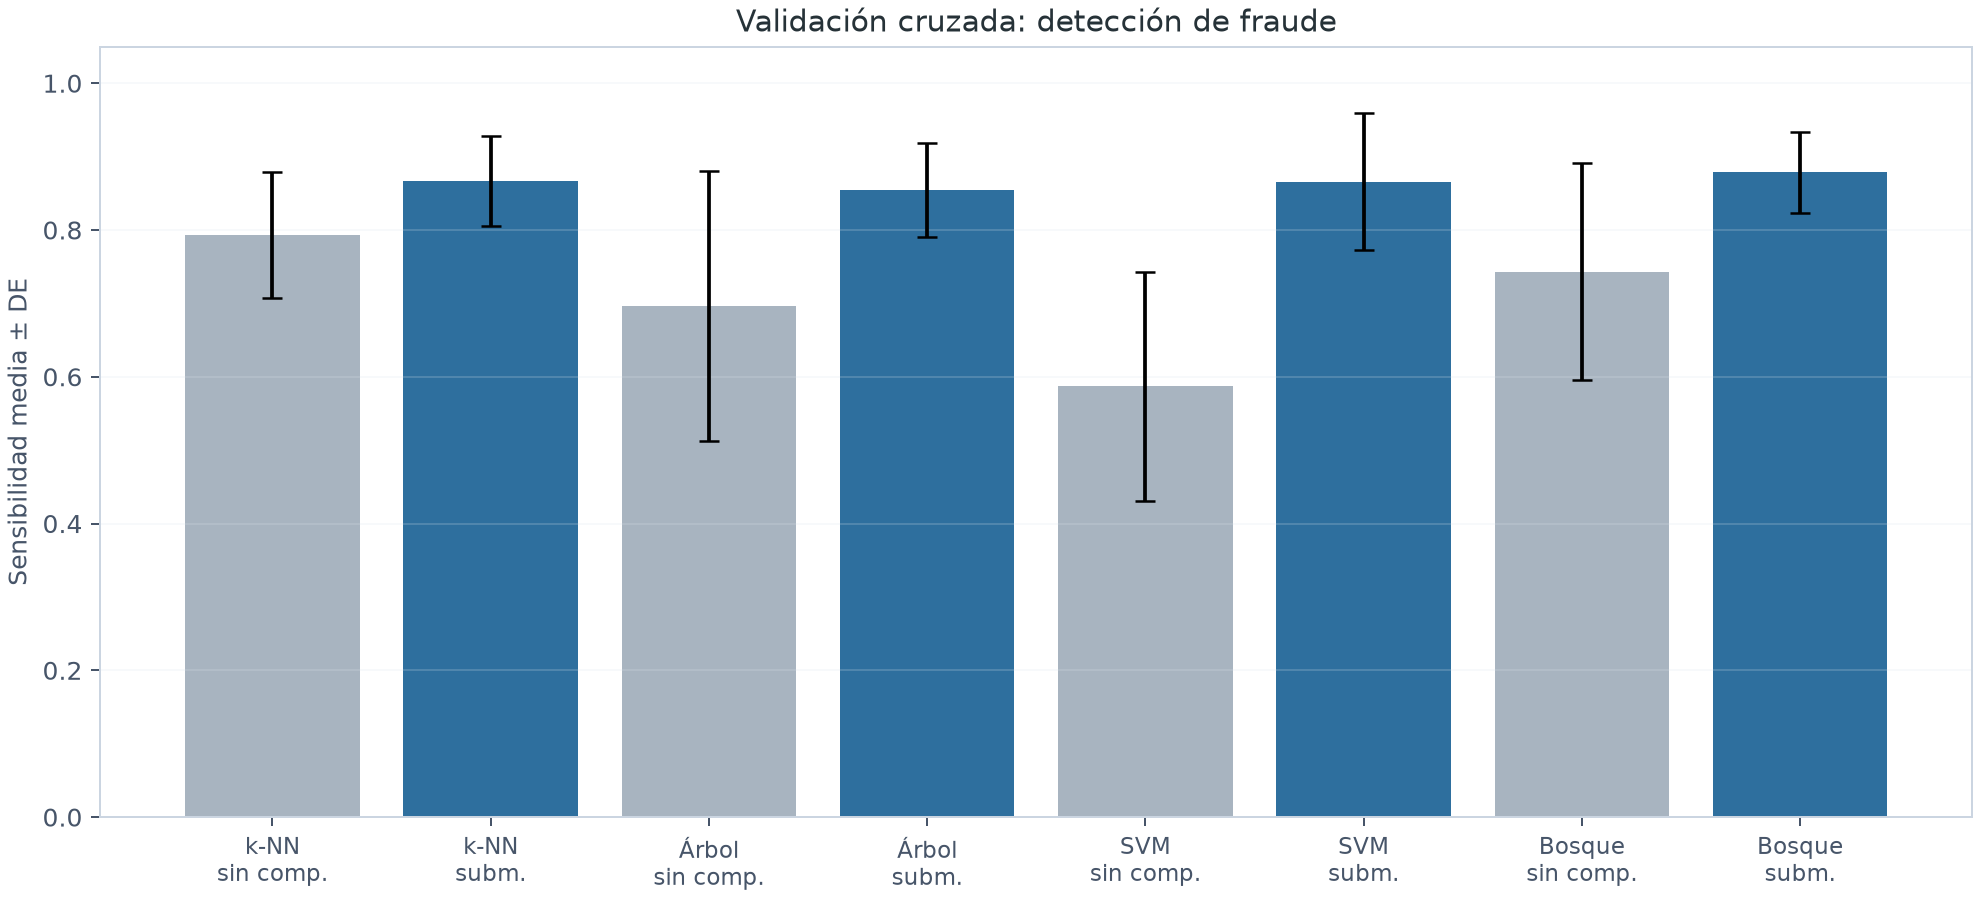
\includegraphics[width=0.96\textwidth,height=0.75\textheight,keepaspectratio]{sensibilidad_validacion.png}

  \vspace{0.1cm}\small Barras: media de cinco pliegues. Líneas: una desviación estándar.
\end{frame}

% 8. Sensibilidad y FNR
\begin{frame}{Prueba reservada: sensibilidad y falsos negativos}
  \centering
  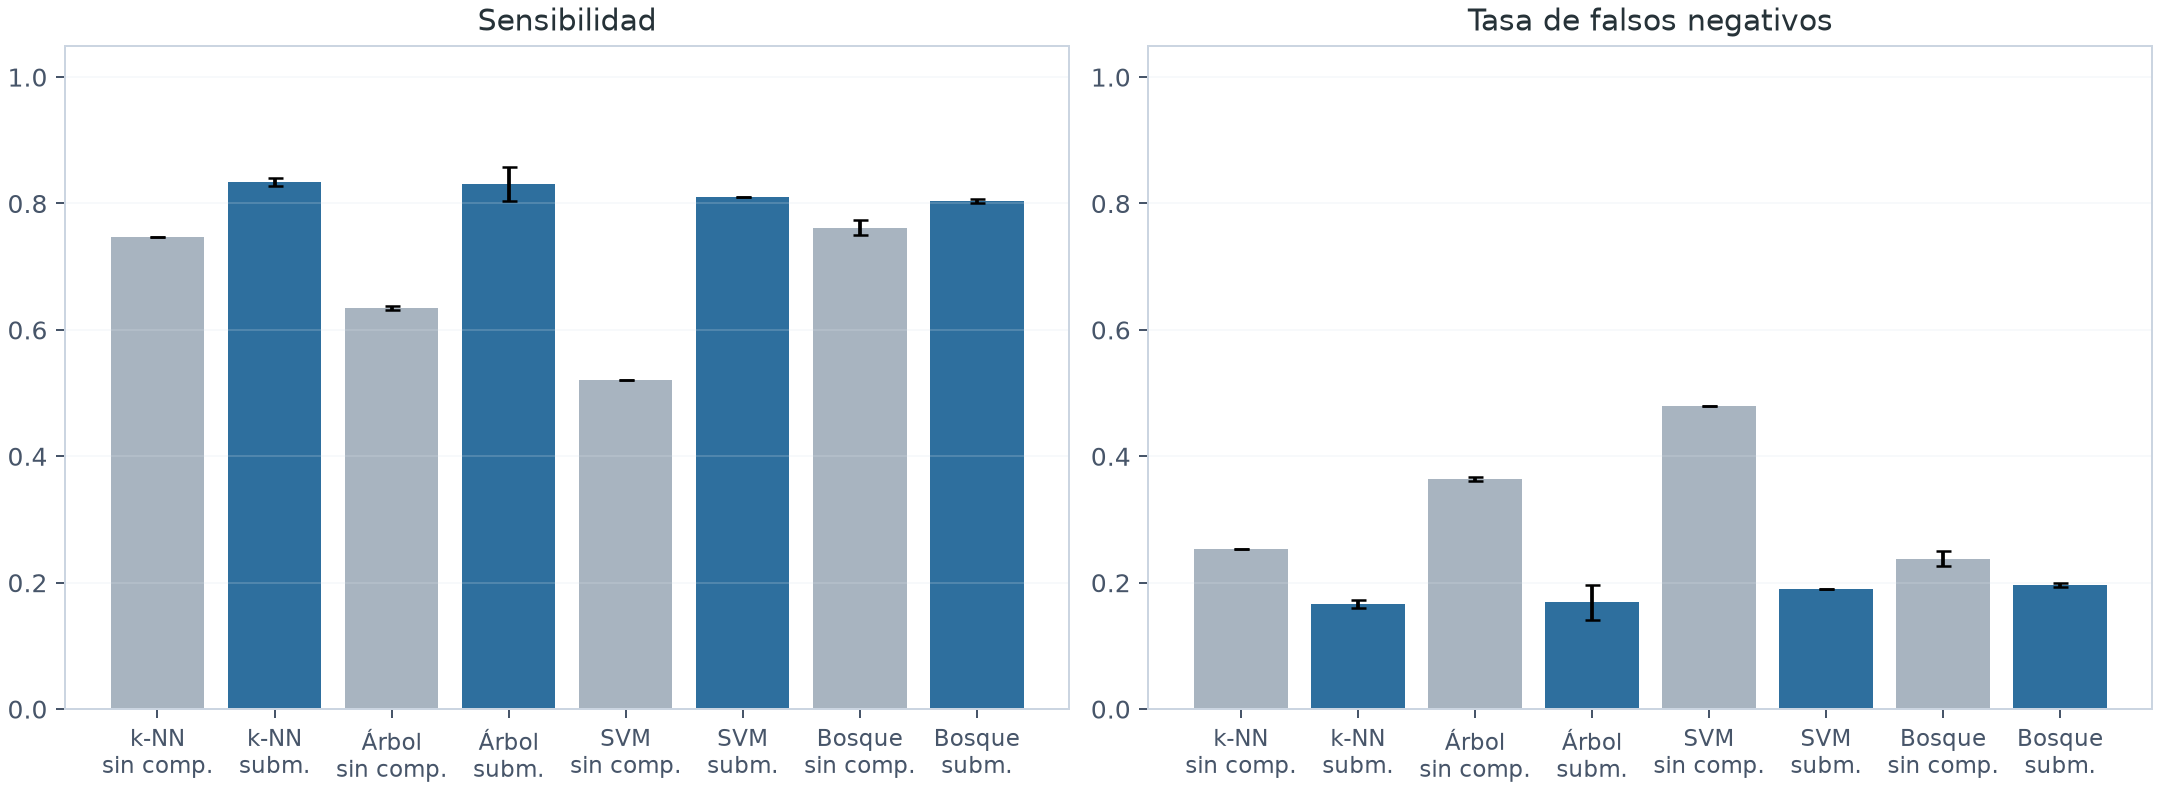
\includegraphics[width=0.96\textwidth,height=0.76\textheight,keepaspectratio]{sensibilidad_fnr_prueba.png}

  \vspace{0.05cm}\small Media $\pm$ desviación estándar entre cinco semillas; el mismo test se usa en todas las repeticiones.
\end{frame}

% 9. Precisión y especificidad
\begin{frame}{Detectar más fraudes genera más alertas}
  \centering
  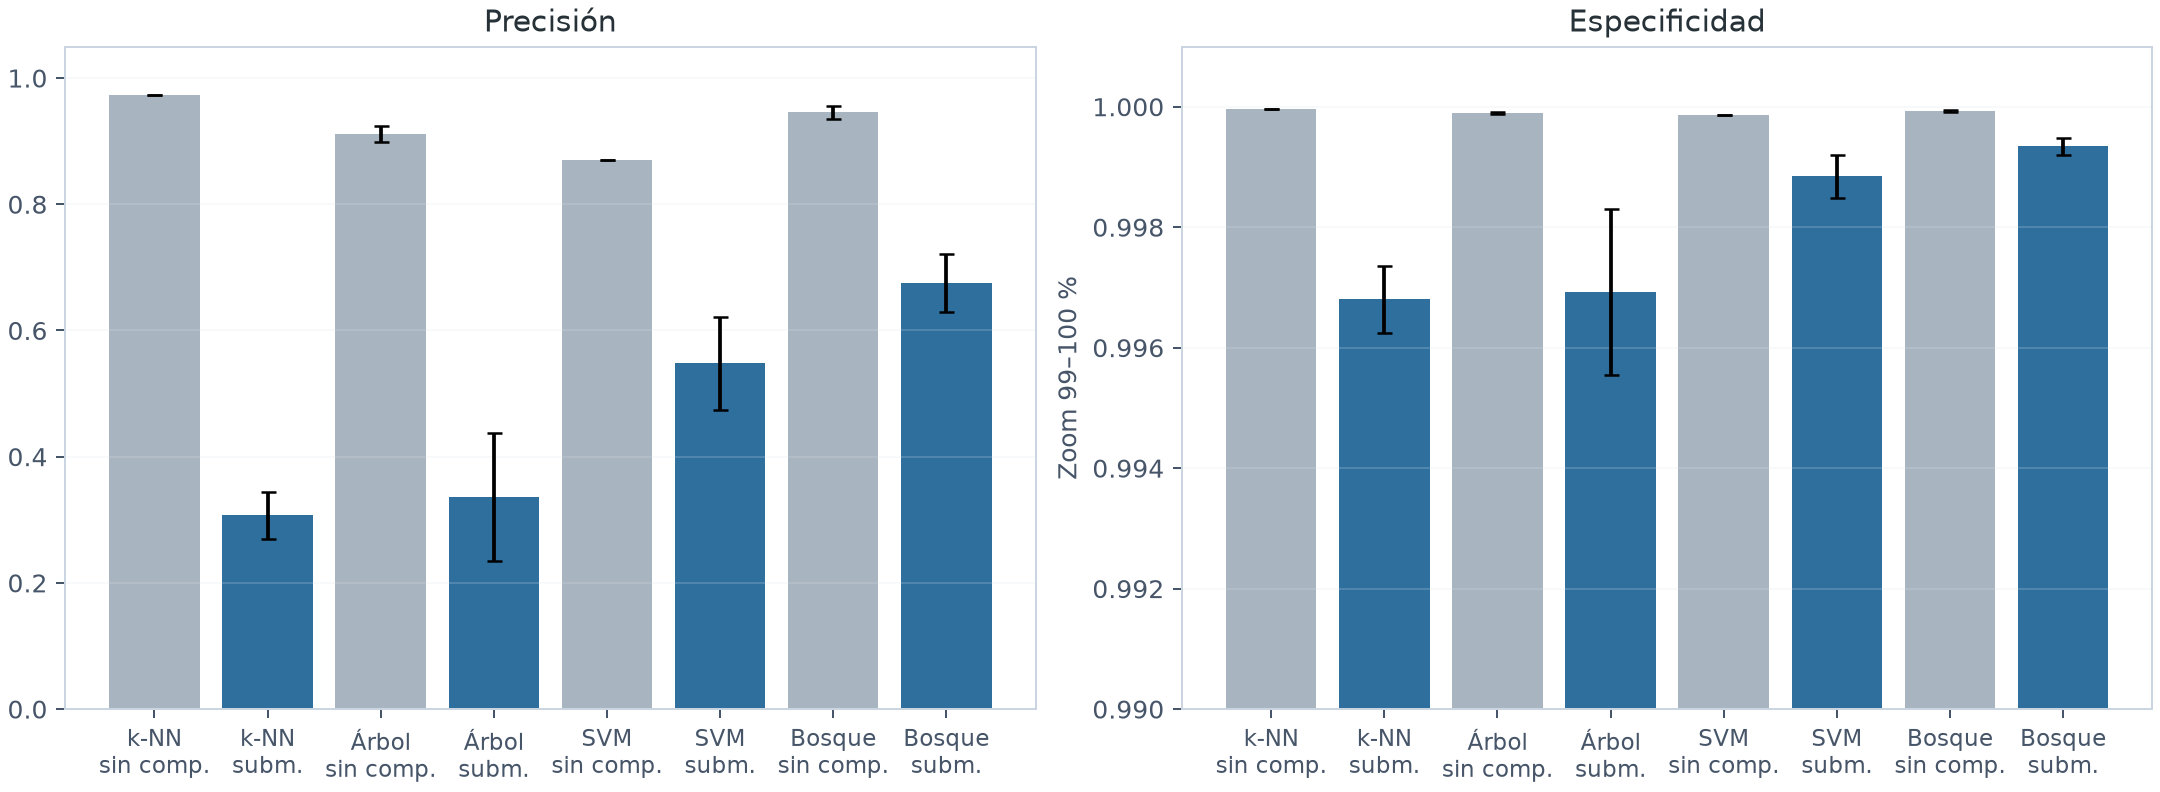
\includegraphics[width=0.96\textwidth,height=0.76\textheight,keepaspectratio]{precision_especificidad_prueba.png}

  \vspace{0.05cm}\small El submuestreo eleva la sensibilidad y aumenta las falsas alarmas; la precisión muestra ese costo.
\end{frame}

% 10. Matriz de confusión
\begin{frame}{Matriz de confusión de la configuración elegida}
  \begin{columns}[c,onlytextwidth]
    \column{0.54\textwidth}
      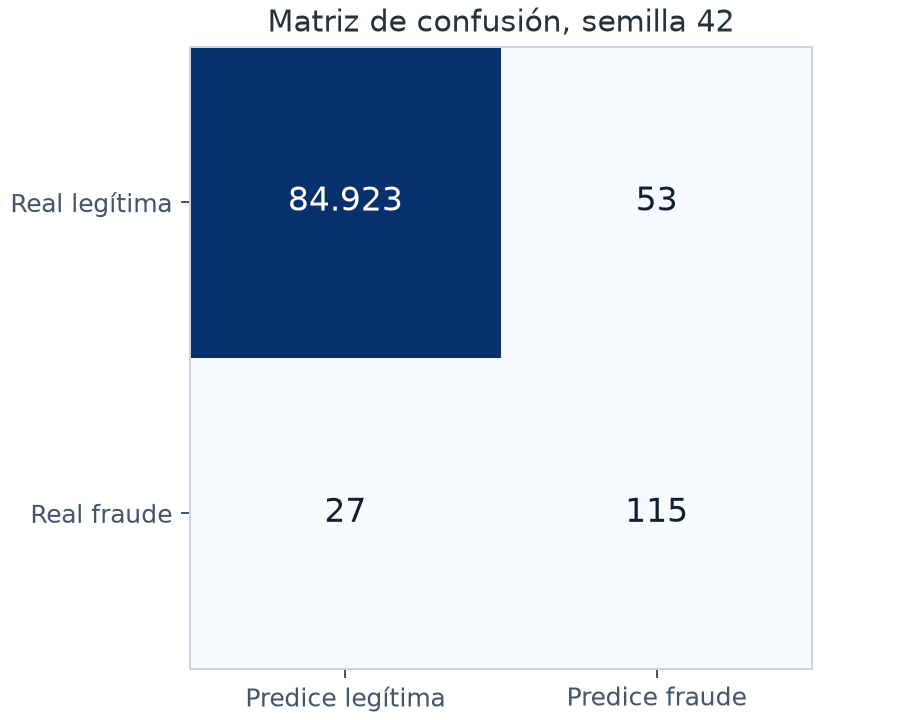
\includegraphics[width=\linewidth,height=0.61\textheight,keepaspectratio]{matriz_confusion_seleccion_cv.png}
    \column{0.42\textwidth}
      \begin{columns}[T,onlytextwidth]
        \column{0.48\textwidth}
          \metricbox{115}{fraudes detectados (TP)}
          \vspace{0.2cm}
          \metricbox{27}{fraudes omitidos (FN)}
        \column{0.48\textwidth}
          \metricbox{53}{falsas alarmas (FP)}
          \vspace{0.2cm}
          \metricbox{84.923}{legítimas reconocidas (TN)}
      \end{columns}
  \end{columns}
  \centering\scriptsize Bosque con submuestreo 1:10; primer ajuste de prueba, semilla 42.
\end{frame}

% 11. Análisis
\begin{frame}{Lectura crítica de los resultados}
  \begin{columns}[T,onlytextwidth]
    \column{0.31\textwidth}\metricbox{99,833\%}{exactitud si todo se predice legítimo en el test; sensibilidad 0\%}
    \column{0.31\textwidth}\metricbox{76,2\% $\to$ 80,4\%}{sensibilidad del bosque sin/con submuestreo}
    \column{0.31\textwidth}\metricbox{67,5\%}{precisión del bosque compensado}
  \end{columns}
  \vspace{0.35cm}
  \begin{itemize}
    \item La exactitud sola oculta los fraudes que el modelo deja pasar.
    \item El árbol compensado detecta 83,1\% de los fraudes, pero su precisión es 33,6\%; el bosque detecta 80,4\% con precisión 67,5\%.
    \item Clasificar todo como fraude marcaría como falsas alarmas las 84.976 transacciones legítimas de prueba.
  \end{itemize}
\end{frame}

% 12. Cierre
\begin{frame}{Conclusiones y límites}
  \begin{columns}[T,onlytextwidth]
    \column{0.32\textwidth}\metricbox{80,4\%}{sensibilidad del modelo elegido en prueba}
    \column{0.32\textwidth}\metricbox{19,6\%}{tasa de falsos negativos}
    \column{0.32\textwidth}\metricbox{67,5\%}{precisión en detección de fraude}
  \end{columns}
  \vspace{0.4cm}
  \begin{block}{Conclusiones}
    \begin{itemize}
      \item CV seleccionó el Random Forest propio con submuestreo por mayor sensibilidad media.
      \item El test contiene solo 142 fraudes; la sensibilidad puede cambiar con pocos casos.
      \item El dataset no identifica transacciones: filas idénticas podrían ser operaciones reales repetidas.
      \item Ambos integrantes deben poder explicar el modelo, las métricas y el costo de las alertas.
    \end{itemize}
  \end{block}
\end{frame}

% 13. Respaldo CV
\begin{frame}{Respaldo: parámetros y resultados de validación}
  \centering\scriptsize Cinco pliegues estratificados compartidos sobre 50.000 filas de entrenamiento.
  \vspace{0.2cm}

  \begin{tabularx}{\textwidth}{>{\raggedright\arraybackslash}p{2.45cm} >{\raggedright\arraybackslash}p{1.8cm} X >{\centering\arraybackslash}p{2.35cm} >{\centering\arraybackslash}p{1.65cm}}
    \rowcolor{FraudPaleBlue}
    \toprule
    \textbf{Modelo} & \textbf{Condición} & \textbf{Mejores parámetros} & \textbf{Sensibilidad $\pm$ DE} & \textbf{Precisión} \\
    \midrule
    k-NN & Sin compensar & $k=3$ & 79,3\% $\pm$ 8,6\% & 91,2\% \\
    \rowcolor{FraudLightGray}
    k-NN & Submuestreo & $k=3$ & 86,6\% $\pm$ 6,1\% & 37,5\% \\
    Árbol & Sin compensar & profundidad 5; hoja 5 & 69,6\% $\pm$ 18,4\% & 79,8\% \\
    \rowcolor{FraudLightGray}
    Árbol & Submuestreo & profundidad 5; hoja 5 & 85,4\% $\pm$ 6,4\% & 18,6\% \\
    SVM lineal & Sin compensar & $C=10$ & 58,7\% $\pm$ 15,6\% & 88,5\% \\
    \rowcolor{FraudLightGray}
    SVM lineal & Submuestreo & $C=10$ & 86,5\% $\pm$ 9,3\% & 21,2\% \\
    Bosque propio & Sin compensar & 21 árboles; profundidad 12 & 74,3\% $\pm$ 14,7\% & 91,6\% \\
    \rowcolor{FraudPaleBlue}\textbf{Bosque propio} & \textbf{Submuestreo} & \textbf{21 árboles; profundidad 6} & \textbf{87,9\% $\pm$ 5,5\%} & \textbf{45,0\%} \\
    \bottomrule
  \end{tabularx}
\end{frame}

% 14. Respaldo prueba
\begin{frame}{Respaldo: métricas completas de prueba}
  \centering\scriptsize Media $\pm$ desviación estándar en puntos porcentuales entre cinco semillas sobre el mismo test fijo.
  \vspace{0.3cm}

  {\scriptsize
  \setlength{\tabcolsep}{3.7pt}
  \begin{tabular}{>{\raggedright\arraybackslash}p{2.0cm} >{\raggedright\arraybackslash}p{1.2cm} c c c c c c}
    \rowcolor{FraudPaleBlue}
    \toprule
    \textbf{Modelo} & \textbf{Condición} & \textbf{Sens.} & \textbf{Espec.} & \textbf{Prec.} & \textbf{F1} & \textbf{Exact.} & \textbf{FNR} \\
    \midrule
    k-NN & Sin comp. & 74,6 $\pm$ 0,0 & 99,996 $\pm$ 0,000 & 97,2 $\pm$ 0,0 & 84,5 $\pm$ 0,0 & 99,95 $\pm$ 0,00 & 25,4 $\pm$ 0,0 \\
    \rowcolor{FraudLightGray}
    k-NN & Subm. & 83,4 $\pm$ 0,6 & 99,681 $\pm$ 0,056 & 30,7 $\pm$ 3,7 & 44,8 $\pm$ 3,9 & 99,65 $\pm$ 0,06 & 16,6 $\pm$ 0,6 \\
    Árbol & Sin comp. & 63,5 $\pm$ 0,3 & 99,990 $\pm$ 0,002 & 91,1 $\pm$ 1,2 & 74,9 $\pm$ 0,4 & 99,93 $\pm$ 0,00 & 36,5 $\pm$ 0,3 \\
    \rowcolor{FraudLightGray}
    Árbol & Subm. & 83,1 $\pm$ 2,7 & 99,692 $\pm$ 0,138 & 33,6 $\pm$ 10,1 & 47,0 $\pm$ 9,6 & 99,66 $\pm$ 0,13 & 16,9 $\pm$ 2,7 \\
    SVM & Sin comp. & 52,1 $\pm$ 0,0 & 99,987 $\pm$ 0,000 & 87,1 $\pm$ 0,0 & 65,2 $\pm$ 0,0 & 99,91 $\pm$ 0,00 & 47,9 $\pm$ 0,0 \\
    \rowcolor{FraudLightGray}
    SVM & Subm. & 81,0 $\pm$ 0,0 & 99,885 $\pm$ 0,036 & 54,8 $\pm$ 7,4 & 65,2 $\pm$ 5,4 & 99,85 $\pm$ 0,04 & 19,0 $\pm$ 0,0 \\
    Bosque & Sin comp. & 76,2 $\pm$ 1,2 & 99,993 $\pm$ 0,002 & 94,6 $\pm$ 1,0 & 84,4 $\pm$ 0,6 & 99,95 $\pm$ 0,00 & 23,8 $\pm$ 1,2 \\
    \rowcolor{FraudPaleBlue}\textbf{Bosque} & \textbf{Subm.} & \textbf{80,4 $\pm$ 0,3} & \textbf{99,935 $\pm$ 0,014} & \textbf{67,5 $\pm$ 4,6} & \textbf{73,3 $\pm$ 2,8} & \textbf{99,90 $\pm$ 0,01} & \textbf{19,6 $\pm$ 0,3} \\
    \bottomrule
  \end{tabular}}
\end{frame}

\end{document}
